Das folgende Kapitel zeigt mögliche Anwendungen von Key Escrow Systemen und deren Alternativen für den Gebrauch von staatlichen Behördern, sowie in der Privatwirtschaft auf.
	
	\subsection{Staatlich}
		% Silvio
Die immer stärker werdenden kryptografischen Verfahren stellen die staatlichen Sicherheitsbehördern vor immer grössere Probleme. Die Anwendung von Verschlüsselung durch Straftäter erschwert die Arbeit der Sicherheutsbehörder enorm. \\
Nach terroristischen Anschlägen werden immer wieder Stimmen laut, welche die Einführung einer Möglichkeit zur Erleichterung der Entschlüsselung von Kommunikationsdaten fordern \cite{insideit} \cite{annabiselli} \cite{denning}. 
Dabei werden immer wieder die selbigen Themen angesprochen:

	\subsubsection{Erstellung eines Key Escrow Systemes}
Die Einführung eines Key Escrow Systemes wäre für jeden Geheimdienst wohl das höchste aller Gefühle. Allerdings hat ein staatliches Key Escrow System politisch einen sehr schweren Standpunkt. Dies liegt vor allem daran, dass ein solches System zu einem gewaltigen Verlust, wenn nicht gerade eine totale Aufgabe der Privatsphäre zur Folge hätte und die Gesellschaft kaum mit einer so drastischen Massnahme einverstanden wäre.\cite {insideit} \\
Fraglich wäre auch der Nutzen des Sytems im Hinsicht auf grössere kriminelle Organisationen. Zu glauben, dass alle Kriminellen Verschlüsselungstools benutzen würden, für welche der Schlüssel im Escrow System hinterlegt ist wäre sehr fraglich. Beispielsweise hat die Terrororganisation Al-Qaida von der Organisation nahestehenden Kryptologen ein eigenes Verschlüsselungssystem entwickeln lassen \cite{denning}. Dass es sich dabei nicht im einen Einzelfall handelt, lasst sich auch stark annehmen.
	
	\subsubsection{Hinterlegung von verwendeten Verschlüsselungsalgorithmen}
Eine nicht so schwerwiegende Alternative zu Key Escrow wäre die Hinterlegung des Verschlüsselungsverfahrens ohne Hinterlegung des verwendeten kryptografischen Schlüssels. Diese Hinterlegung sollte zum Nutzen haben, dass den Strafverfolgungsbehörden die Arbeit etwas erleichtert würde. Dies hätte allerdings auch nur dann einen Nutzen, wenn nur schwächere oder Algorithmen mit einer Sicherheitslücke verwendet werden dürfen. Diese Lücken wären somit auch ein Eigentor für die Sicherheitsbehörden, da sie somit Kriminellen eine weiter Angriffsfläche auf die Bürger bieten würden. \cite{adminch} % KP. 7.3.

	
	\subsubsection{Verbot von alternativen Verschlüsselung}
Mit der Einführung eines Escrow Systemes oder der Einführung einer Hinterlegungspflicht für Algorithmen würde auch dazu führen, dass die Gegenseite, das heisst die Verwendung nicht hinterlegter Schlüssel / Algorithmen, verboten werden müsste. Auf der einen Seite wäre ein solches Verbot sehr schwer durchzusetzten, geschweige überhaupt zu kontrollieren, auf der andern Seite wäre es von der Strafnorm her auch kaum möglich, eine genug hohe Maximalstrafe ansetzen zu können, um grössere kriminelle Organisationen von der illealgen Verwendung der Verschlüsselung abzuwenden. \cite{adminch} \\ %KP 7.3.
Zudem wäre ein solches Verbot auch nur dann vernünftig brauchbar und durchsetzbar, wenn es von der internationalen Gemeinschaft getragen und somit in allen Ländern durchgesetzt würde \cite{denning}. Da der Internationale Weg in Sache Verschlüsselungspolitik in eine andere Richtung weht, zeigt sich darin, dass sich einige Länder, welche in den neunziger Jahren die Kryptografie noch eingeschränkt hatten, in Richtung einer offenen Kryptografiepolitik bewegen. \cite{clipperchip} \cite{adminch} \\ % 7.2.3
Eine Einführung eines solchen Verbotes würde einen Staat Interational stark ins Abseits setzten und das Verbot wäre somit auch kaum duchsetzbar.
		
	\subsection{Firmenintern}
Das nachfolgende Kapitel gibt einen Überblick über die Problembereiche beim Key Management von Firmen und zeigt auf, inwiefern Hintertüren für staatliche Eingriffe in Software eingebaut werden können.

	\subsubsection{Key Management Systeme (KMS)}
Das zentrale Verwalten und hinterlegen von Schlüsseln ist für grössere Firmen eine Notwendigkeit. \\
Geschäftskritische Daten sollten wenn immer verschlüsselt werden. Um den Überblick über die verwendeten Schlüssel zu bewahren, werden Key Management Systeme (KMS) eingesetzt.
Mit diesen Systemen lassen sich folgende Problembereiche addressieren:
\begin{itemize}
	\item Datensicherheit durch Verschlüsselung gewährleisten
	\item Zentrales Verwalten und Administrieren von Schlüsseln
	\item Entschlüsseln von Geschäftsdaten von Mitarbeitenden bei Tod oder Abwesenheit
	\item Entschlüsseln von Geschäftsdaten bei untreuen Mitarbeitern
  \item Überwachung von Mitarbeitern
  \item Verwalten und verteilen von Softwarelizenzen
\end{itemize}
	

	\subsection{Exemplarisches Beispiel: Clipper Chip}
\begin{figure}[H]
	\centering
	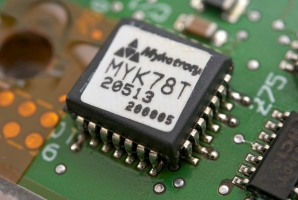
\includegraphics[width=.8\textwidth]{clipper-chip.jpg}
	\caption{MYK78T Clipper Chip (1993)}
	\label{fig:clipper-chip}
\end{figure}
Ein exemplarisches Beispiel für staatliches erzwungenes Key Escrow ist der sogenannte Clipper Chip aus dem Jahre 1993. Dieser wurde von der NSA in Zusammenarbeit den US-Behörden entwickelt. \\
Der Clipper Chip bietet hardwaremässige Verschlüsselung mit einer staatlich eingebauten Hintertür. Die Behörden konnten die Verschlüsselungsmechanismen für jeden Clipper Chip rückgängig machen und so an die ursprünglichen Daten kommen. \\
Eingesetzt werden sollte der Chip bei verschlüsselter Telefonie.\\
Designed wurde der Chip von Mykrotronx, hergestellt von VLSI Technology Inc. \\

	\subsubsection{Verschlüsselung mit Backdoor}
Der Clipper Chip verwendet zur Verschlüsselung den Skipjack-Verschlüsselungsalgorithmus welcher dem DES-Algorithmus ähnelt. Entwickelt wurde Skipjack von der NSA und wurde bis zur Veröffentlichung im Jahre 1998 unter Verschluss gehalten. \cite{skipjack_wikipedia}


Um Missbrauch der Behörden einzudämmen, wurde d


	\subsection{Recovery Agents und Trusted Third Parties}
Bei Key Escrow handelt es sich um ein Verfahren um Schlüssel für den späteren Gebrauch zu hinterlegen. Key Recovery ist der Prozess der Schlüssel anhand bestehender Daten rekonstruiert.
\\
Falls Key Recovery, beziehungsweise Key Escrow von zwei Parteien erwünscht ist, wird meist eine Trusted Third Party als unabhängige Kontroll- und Aufsichtsinstanz hinzugezogen.
\\
Die ausführende Instanz für Key Escrow und Key Recovery ist als Teil einer Trusted Thir Party der Recovery Agent.
		\subsubsection{Recovery Agent als Man in the Middle bei symmetrisch verschlüsselter Kommunikation}
Die beiden nachfolgenden Abbildungen illustrieren eine einfache funktionsweise eines Recovery Agent gemäss \cite{isss}.
\\
In Abbildung \ref{fig:recovery-agent-aufbau} werden zwei kommunizierende Computer dargestellt. \textit{A} nimmt die Rolle des Senders und \textit{B} die Rolle des Empfängers ein. Sie nutzen zur Verschlüsselung der Nachricht ein symmetrisches Chiffrierverfahren. Der genutzte Schlüssel $K_{AB}$ wurde bereits ausgetauscht. \textit{A} erstellt die Nachricht $M$ und chiffriert sie mittels $E(K_{AB},M)=M_{C}$. Die chriffrierte Nachricht $M_{C}$ wird über den Datenkanal übertragen und von \textit{B} empfangen. Nach Dechiffrierung mittels $D(K_{AB},M_{C})=M$ kann die Nachricht $M$ von \textit{B} weiterverarbeitet werden.
\begin{figure}[H]
	\centering
	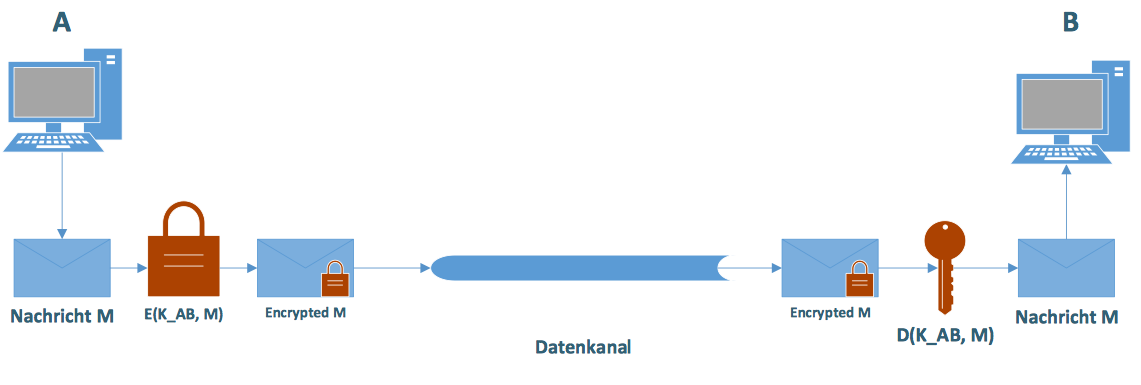
\includegraphics[width=.8\textwidth]
		{recovery-agent-aufbau.png}
	\caption{Symmetrische Verschlüsselung einer Kommunikation}
	\label{fig:recovery-agent-aufbau}
\end{figure}
Abbildung \ref{fig:recovery-agent-mitm} erweitert die symmetrisch verschlüsselte Kommunikation von \textit{A} und \textit{B} mit einem Recovery Agenten \textit{RA}.
\\
Dieser besitzt ebenfalls einen Schlüssel $K_{RA}$. Beim Senden der Nachricht $M$ wird ebenfalls der chiffrierte Schlüssel $E(K_{RA},K_{AB})=C_{K_{AB}}$ von \textit{A} übertragen. Der Recovery Agent \textit{RA} hört die chiffrierte Nachricht $M_{C}$ und den chiffrierten Schlüssel $C_{K_{AB}}$ vom Datenkanal ab. Er dechiffriert den Schlüssel von \textit{A} und \textit{B} mittels $D(K_{RA}, C_{K_{AB}})=K_{AB}$ und kann somit auch die chiffrierte Nachricht $M_{C}$ dechiffrieren.
\begin{figure}[H]
	\centering
	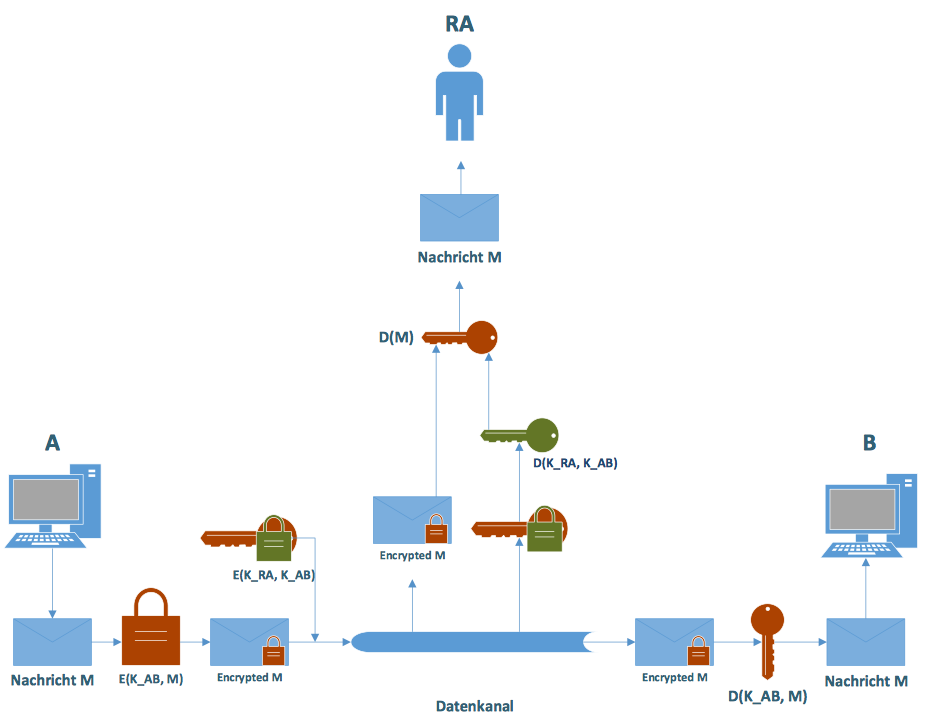
\includegraphics[width=.8\textwidth]
		{recovery-agent-mitm.png}
	\caption{Recovery Agent als Man in the Middle}
	\label{fig:recovery-agent-mitm}
\end{figure}
